\documentclass[border=3pt]{standalone}
\usepackage{amsmath,pgfplots}
\pgfplotsset{compat=1.18}
\begin{document}
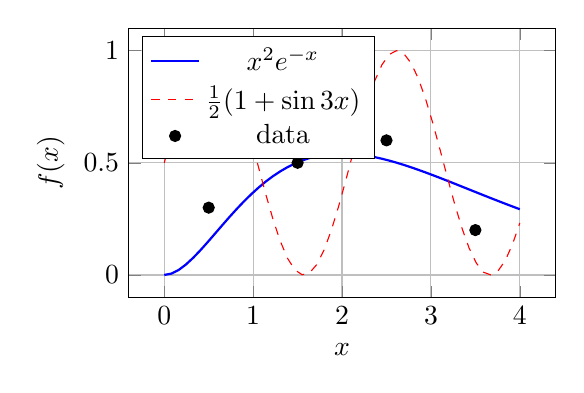
\begin{tikzpicture}
  \begin{axis}[width=7cm,height=5cm,xlabel={$x$},ylabel={$f(x)$},legend pos=north west,grid=major]
    \addplot[blue,thick,domain=0:4,samples=50] {x^2*exp(-x)};
    \addplot[red,dashed,domain=0:4,samples=50] {0.5*sin(deg(3*x))+0.5};
    \addplot[only marks,mark=*] coordinates {(0.5,0.3) (1.5,0.5) (2.5,0.6) (3.5,0.2)};
    \legend{$x^2e^{-x}$,$\tfrac12(1+\sin 3x)$,data}
  \end{axis}
\end{tikzpicture}
\end{document}
